\documentclass[12pt, a4paper]{report}
\usepackage[utf8]{inputenc}
\newcommand\preamble{
    \usepackage[italian]{babel}
    \usepackage{geometry}
    \usepackage{amsmath}
    \usepackage{amssymb}
    \usepackage{graphicx}
    \usepackage{ulem}
    \geometry{margin=2cm}
    \usepackage{listings}
    \usepackage{titling}
    \let\olditemize\itemize
    \renewcommand\itemize{\olditemize\setlength\itemsep{0em}}
}
% Definizione delle variabili
\newcommand{\imagePath}{Immagini/logoUni.png}

% Definizione del comando per la pagina di titolo con argomenti
\newcommand{\customTitlePage}[5]{
    \newcommand{\courseTitle}{#1}
    \newcommand{\authorName}{#2}
    \newcommand{\academicYear}{#3}
    \newcommand{\universityName}{#4}
    
    \begin{titlepage}
        \centering
        \includegraphics[width=0.5\textwidth]{\imagePath}\par\vspace{1cm}
        {\scshape\LARGE \universityName \par}
        \vspace{1.5cm}
        {\huge\bfseries \courseTitle \par}
        \vspace{2cm}
        {\Large\itshape \authorName \par}
        \vfill
        \academicYear
    \end{titlepage}
}
  
\preamble

\begin{document}
\customTitlePage{Fondamenti dell'Elaborazione di Segnali e Immagini}{Lorenzo Vaccarecci}{Anno Accademico 2024/2025}{Università degli Studi di Genova}
\newpage
\tableofcontents
\chapter{Introduzione}
\section{Segnali 1D e 2D}
\subsection{Segnali 1D}
Un segnale 1D descrive una grandezza fisica che varia nel tempo, e può essere visto come una funzione di una variabile indipendente: 
\begin{equation*}
    g = f(t)
\end{equation*}
dove $g$ è il valore della grandezza fisica (variabile \textbf{dipendente}), $f$ è la funzione (continua o discreta) e $t$ è la variabile indipendente.\\
Esempi di segnali 1D sono:
\begin{itemize}
    \item Segnali audio: come ad esempio la musica o il parlato.
    \item Segnali ECG
    \item Segnali EEG
    \item Sensori inerziali
    \item \dots
\end{itemize}
\subsection{Segnali 2D}
Un segnale 2D descrive una grandezza fisica che varia nello spazio, e può essere visto come una funzione di due variabili indipendenti.\\
Esempi di segnali 2D sono:
\begin{itemize}
    \item Immagini: utilizzeremo questo termine per indicare una foto a colori o a scala di grigi (ci concentreremo su queste).
    \item Immagini biomediche: come ad esempio le radiografie, le ecografie oppure quelle di una risonanza.
    \item Immagini termiche
    \item Immagini satellitari
    \item Immagini microscopiche
    \item \dots
\end{itemize}
Ciò che hanno in comunque tutte queste immagini è che hanno una matrice di pixel che rappresenta qualcosa, nel nostro caso ogni pixel rappresenta l'intensità luminosa nella posizione $(r,c)$ della matrice.
\section{Segnali a tempo continuo o discreto}
\begin{equation*}
    g = f(t)
\end{equation*}
\subsection{Segnali a tempo continuo}
Nei segnali a tempo continuo $t$ assume valori reali
\begin{figure}[h!]
    \centering
    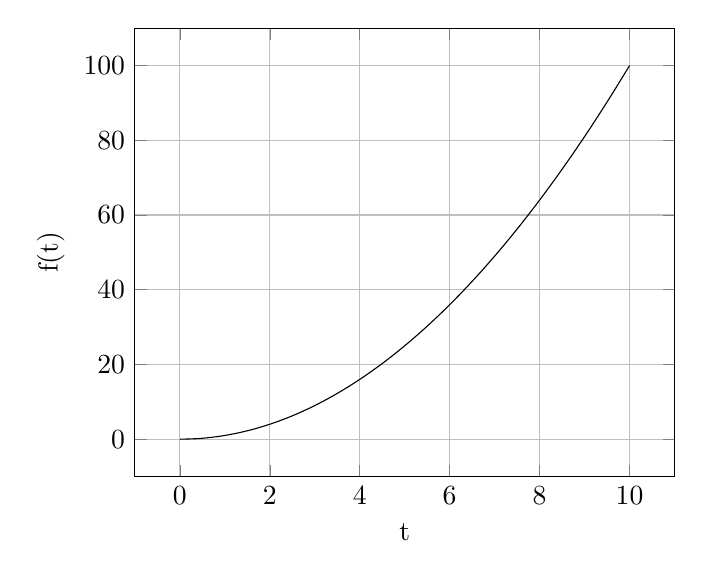
\begin{tikzpicture}
        \begin{axis}[
            xlabel={t},
            ylabel={f(t)},
            grid=major,
        ]
        \addplot[smooth, domain=0:10] {x^2};
        \end{axis}
    \end{tikzpicture}
    \caption{Posso conoscere il valore del segnale in ogni istante di tempo}
\end{figure}
\subsection{Segnali a tempo discreto}
Nei segnali a tempo discreto $t$ assume valori in un sottoinsieme discreto dei numeri reali, come risultato di un'operazione chiamata \textbf{campionamento}.
\begin{figure}[h!]
    \centering
    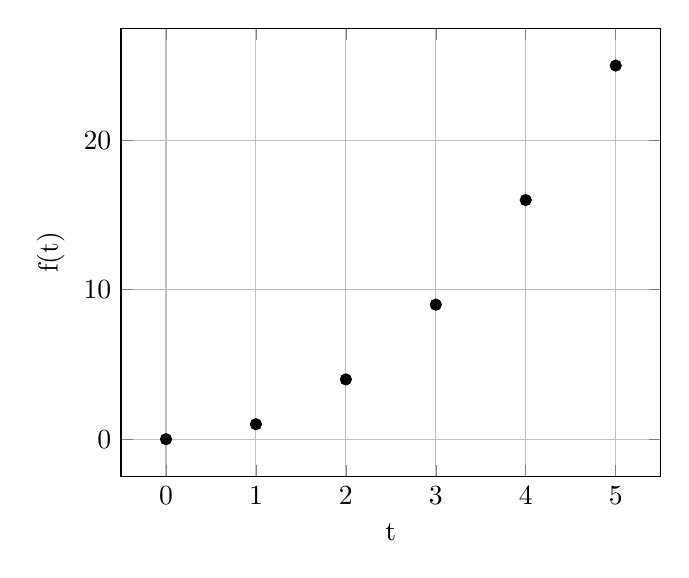
\begin{tikzpicture}
        \begin{axis}[
            xlabel={t},
            ylabel={f(t)},
            grid=major,
            only marks,
        ]
        \addplot[mark=*] coordinates {
            (0,0) (1,1) (2,4) (3,9) (4,16) (5,25)
        };
        \end{axis}
    \end{tikzpicture}
    \caption{Posso conoscere il valore del segnale in certi istanti di tempo}
\end{figure}
\section{Segnali a valori continui o discreti}
\subsection{Segnali a valori continui}
Nei segnali a valori continui $g$ assume valori reali.
\subsection{Segnali a valori discreti}
Nei segnali a valori discreti $g$ assume valori in un sottoinsieme discreto dei numeri reali, come risultato di un'operazione chiamata \textbf{quantizzazione}.
\begin{figure}[h!]
    \centering
    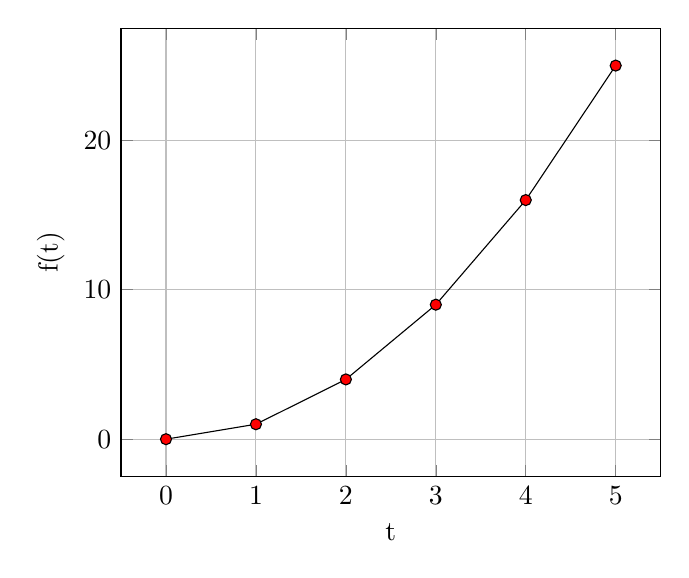
\begin{tikzpicture}
        \begin{axis}[
            xlabel={t},
            ylabel={f(t)},
            grid=major,
        ]
        \addplot[mark=*,mark options={fill=red}, domain=0:5, samples=6] {x^2};
        \end{axis}
    \end{tikzpicture}
    \caption{In rosso i valori \textbf{discreti} di g}
\end{figure}
\section{Analogico e digitale}
\begin{itemize}
    \item \textbf{Segnali analogici}: sono continui sia nel tempo che nei valori.
    \item \textbf{Segnali digitali}: sono discreti sia nel tempo che nei valori.
\end{itemize}
\begin{figure}[h!]
    \centering
    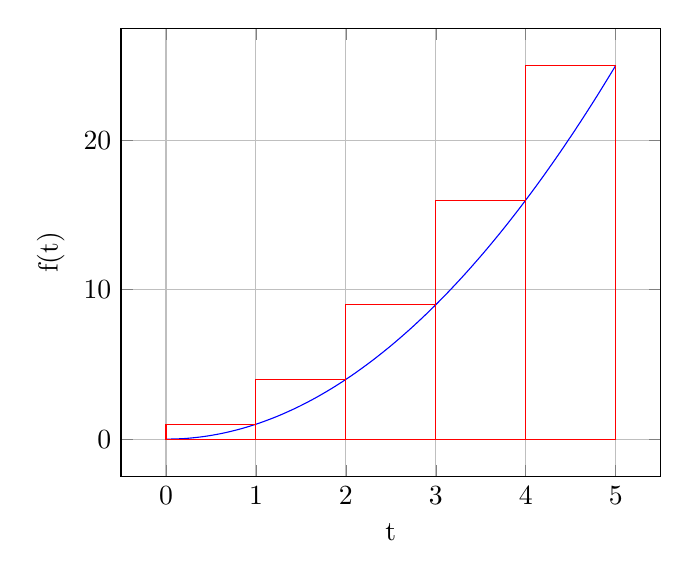
\begin{tikzpicture}
        \begin{axis}[
            xlabel={t},
            ylabel={f(t)},
            grid=major,
        ]
        \addplot[smooth, domain=0:5, color=blue] {x^2};
        \draw[draw=red] (axis cs:0,0) rectangle (axis cs:1,1);
        \draw[draw=red] (axis cs:1,0) rectangle (axis cs:2,4);
        \draw[draw=red] (axis cs:2,0) rectangle (axis cs:3,9);
        \draw[draw=red] (axis cs:3,0) rectangle (axis cs:4,16);
        \draw[draw=red] (axis cs:4,0) rectangle (axis cs:5,25);
        \end{axis}
    \end{tikzpicture}
    \caption{Segnale analogico in blu e segnale digitale in rosso}
\end{figure}
\section{Campionamento}
\begin{equation*}
    v_{s} = \frac{1}{\tau}
\end{equation*}
Dove $v_{s}$ è la frequenza di campionamento e $\tau$ è l'ampiezza dell'intervallo di campionamento. Ovviamente se $\tau$ si avvicina a 0 allora il grafico risultante $f(n\tau)$ sarà più preciso (e vicino a quello continuo) ma userà più risorse per memorizzare i dati.
\subsection{Frequenza ideale di campionamento}
Bisogna stare attenti a non campionare a frequenze troppo basse, altrimenti si incorre nel fenomeno chiamato \textbf{punto di rottura} ossia il grafico risultante apparirà diverso da quello originale.
\begin{figure}[h!]
    \centering
    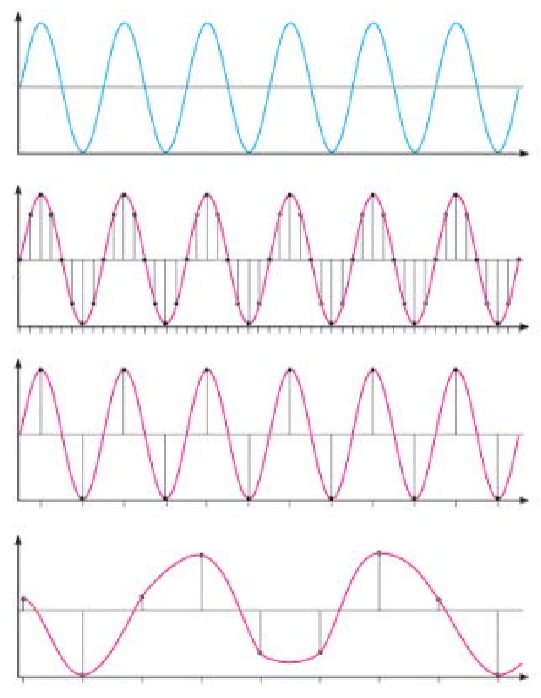
\includegraphics[width=0.5\textwidth]{Immagini/campionamento.png}
\end{figure}
\\Come possiamo vedere dalla figura l'ultimo grafico risulta essere diverso da quello azzurro (originale), questo perché la frequenza di campionamento non è sufficientemente alta in questo caso si è verificato un punto di rottura.
\newpage
\section{Quantizzazione}
\begin{figure}[h!]
    \centering
    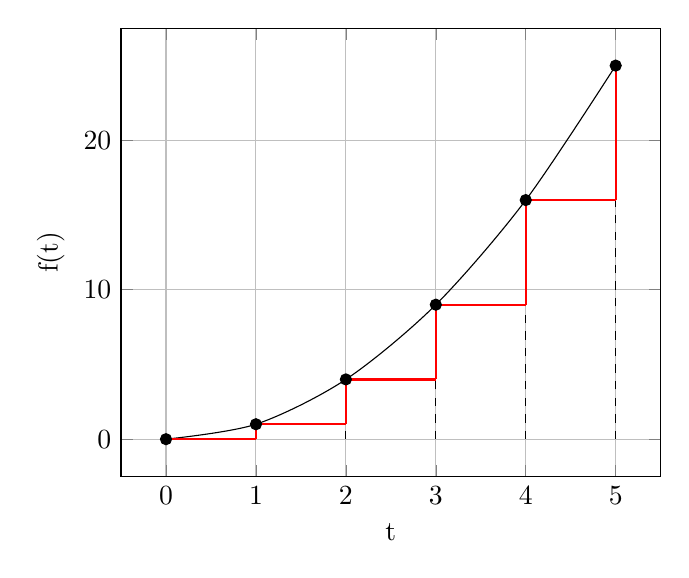
\begin{tikzpicture}
        \begin{axis}[
            xlabel={t},
            ylabel={f(t)},
            grid=major,
        ]
        \addplot[smooth, domain=0:5, mark=*, samples=6] {x^2};
        \draw[dashed] (axis cs:1,0) -- (axis cs:1,1);
        \draw[dashed] (axis cs:2,0) -- (axis cs:2,4);
        \draw[dashed] (axis cs:3,0) -- (axis cs:3,9);
        \draw[dashed] (axis cs:4,0) -- (axis cs:4,16);
        \draw[dashed] (axis cs:5,0) -- (axis cs:5,25);
        \draw[draw=red, thick] (axis cs:0,0) -- (axis cs:1,0);
        \draw[draw=red, thick] (axis cs:1,0) -- (axis cs:1,1);
        \draw[draw=red, thick] (axis cs:1,1) -- (axis cs:2,1);
        \draw[draw=red, thick] (axis cs:2,1) -- (axis cs:2,4);
        \draw[draw=red, thick] (axis cs:2,4) -- (axis cs:3,4);
        \draw[draw=red, thick] (axis cs:3,4) -- (axis cs:3,9);
        \draw[draw=red, thick] (axis cs:3,9) -- (axis cs:4,9);
        \draw[draw=red, thick] (axis cs:4,9) -- (axis cs:4,16);
        \draw[draw=red, thick] (axis cs:4,16) -- (axis cs:5,16);
        \draw[draw=red, thick] (axis cs:5,16) -- (axis cs:5,25);
        \end{axis}
    \end{tikzpicture}
\end{figure}
Partendo da una funzione $f(n\tau)$ quantizziamo i valori associando ad ogni valore $x$ il valore numerico $xk$ che è più vicino ad $x$.
\section{Riepilogo digitalizzazione}
\begin{figure}[h!]
    \centering
    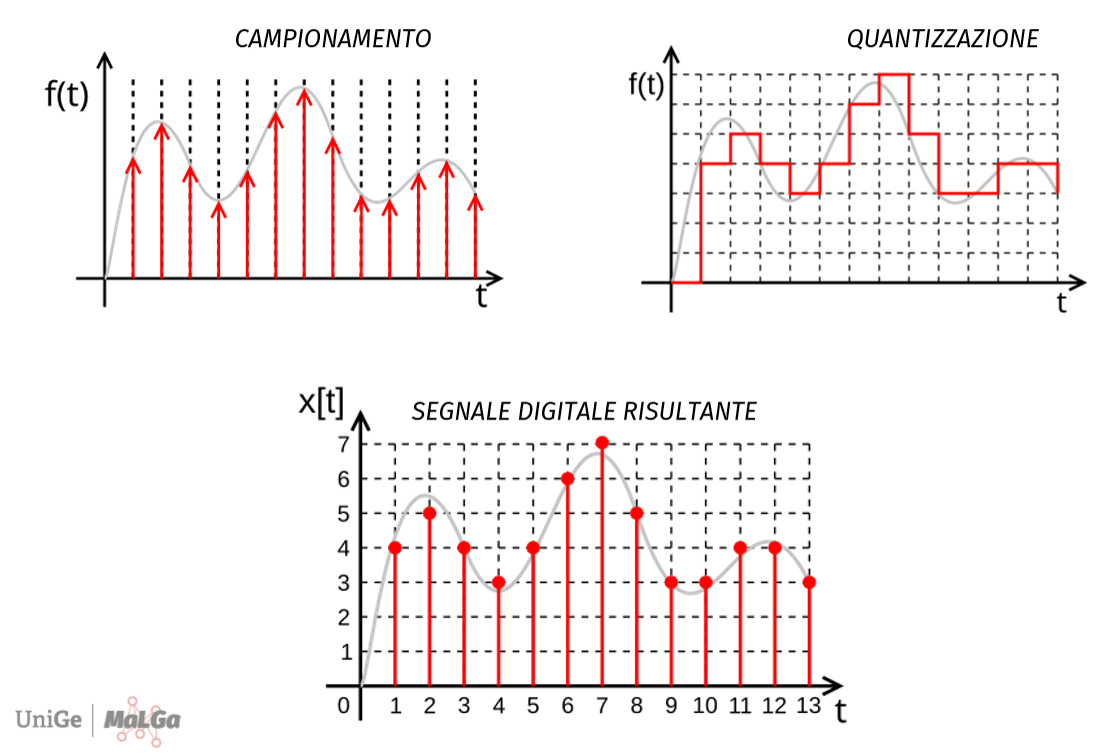
\includegraphics[width=\textwidth]{Immagini/digitalizzazione.png}
\end{figure}
\section{Ripasso: trasformazioni di segnali (1D)}
\subsection{Traslazione}
\begin{equation*}
    f(t-t_{0})
\end{equation*}
\subsection{Scalatura}
\begin{equation*}
    f(\alpha t)
\end{equation*}
\begin{itemize}
    \item $\alpha > 1$ : compressione
    \item $0 < \alpha < 1$ : rilassamento
\end{itemize}
\subsection{Segnali "notevoli"}
\begin{itemize}
    \item \textbf{Segnale rettangolare}: \begin{equation*}
        f(t) = \begin{cases} 
        1 & \lvert t \rvert < \frac{1}{2} \\
        0 & \lvert t \rvert > \frac{1}{2}
    \end{cases}
    \end{equation*}
    \item \textbf{Segnale gradino}: \begin{equation*}
        f(t) = \begin{cases} 
        1 & t > 0 \\
        0 & t < 0
    \end{cases}
    \end{equation*}
    \item \textbf{Segnale impulsivo (o delta di Dirac)}: \begin{equation*}
        \delta(t) = \begin{cases} 
        \infty & t = 0 \\
        0 & t \neq 0
    \end{cases}
    \end{equation*}
\end{itemize}
\subsection{Treno di impulsi equispaziati}
\begin{equation*}
    \delta_{r}(t) = \sum_{n=-\infty}^{+\infty} \delta(t-n\tau)
\end{equation*}
\subsubsection{Campionamento}
Moltiplichiamo il segnale $f(t)$ per il treno di impulsi equispaziati e otteniamo:
\begin{equation*}
    f_{s}(t) = f(t) \cdot \delta_{r}(t) = \sum_{n=-\infty}^{+\infty} f(n\tau) \delta(t-n\tau)
\end{equation*}
\chapter{La trasformata di Fourier}
\section{Introduzione}
Le funzioni continue e periodiche possono essere rappresentate come somme (pesate) di seni e coseni e grazie alla serie di Fourier possiamo ottenere una rappresentazione alternativa del segnale periodico e uno strumento utile per approssimarlo (con compressione e riduzione del rumore).\\
\textbf{Perchè Fourier?} Per capire meglio il segnale.
\begin{center}
    \begin{figure}[h!]
        \centering
        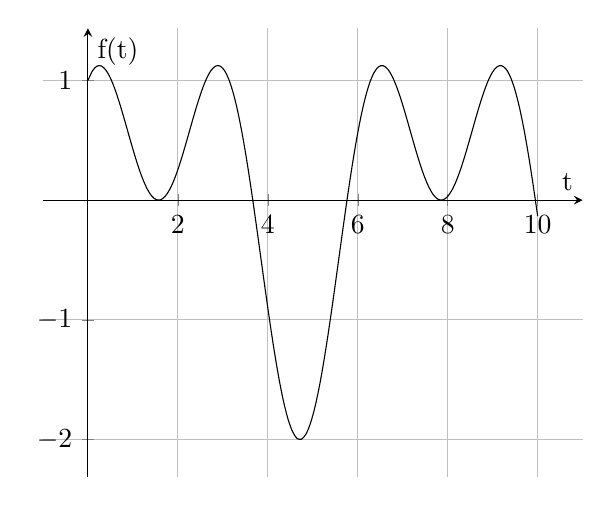
\begin{tikzpicture}
            \begin{axis}[
                xlabel={t},
                ylabel={f(t)},
                grid=major,
                axis lines=middle,
                enlargelimits,
            ]
            \addplot[smooth, domain=0:10, samples=100] {sin(deg(x)) + cos(deg(2*x))};
            \end{axis}
        \end{tikzpicture}
        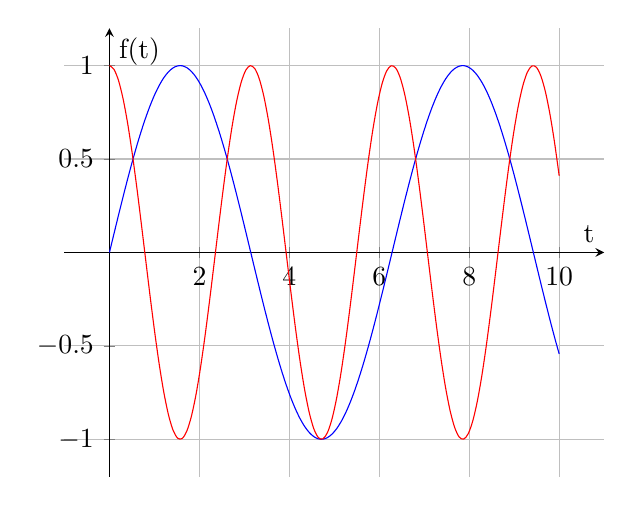
\begin{tikzpicture}
            \begin{axis}[
                xlabel={t},
                ylabel={f(t)},
                grid=major,
                axis lines=middle,
                enlargelimits,
            ]
            \addplot[smooth, domain=0:10, samples=100, color=blue] {sin(deg(x))};
            \addplot[smooth, domain=0:10, samples=100, color=red] {cos(deg(2*x))};
            \end{axis}
        \end{tikzpicture}
        \caption{A sinistra il segnale originale, a destra la sua rappresentazione come somma di una sinusoide e una cosinusoide}
    \end{figure}    
\end{center}
Una funzione continua e periodica può essere descritta attraverso una serie di sinusoidi e possiamo considerare una rappresentazione alternativa del segnale l'insieme dei coefficienti (pesi) dei sinusoidi.
\begin{center}
    \textbf{Immagine qui}
\end{center}
\section{Matematicamente}
Consideriamo una funzione $f(t)$ continua e periodica di periodo $\tau$
\begin{equation*}
    f(t) = a_{0} + \sum_{k=1}^{+\infty} \left(a_{k} \cos\left(\frac{2\pi k t}{\tau}\right) + b_{k} \sin\left(\frac{2\pi k t}{\tau}\right)\right)
\end{equation*}
Dove $a$ e $b$ sono i coefficienti.\\
Riscriviamo applicando la formula di Eulero $e^{j\theta} = \cos(\theta) + j\sin(\theta)$ dove $j = \sqrt{-1}$ immaginario:
\begin{equation*}
    f(t) = \sum_{k=-\infty}^{+\infty} c_{k} e^{j\frac{2\pi k t}{\tau}}
\end{equation*}
\begin{equation*}
    c_{k} = \frac{1}{\tau} \int_{-\frac{\tau}{2}}^{\frac{\tau}{2}} f(t) e^{-j\frac{2\pi k t}{\tau}} dt
\end{equation*}
\subsection{Trasformata di Fourier Discreta}
\textbf{N.B.}: $f(t)$ funzione continua, $f[n]$ funzione discreta.
\begin{equation*}
    f[n] = \sum_{k=0}^{N-1} F[k] e^{j\frac{2\pi k n}{N}}
\end{equation*}
Dove $F[x]\equiv c_{k}$. La sommatoria è finita perchè nel caso di funzione discreta non mi occorrono infiniti sinusoidi per ricostruire tutti i dettagli.\\
Data una funzione discreta e finita $f[n]$ con $N$ campioni, la sua \textbf{DFT} è
\begin{equation*}
    F(k) = \sum_{n=0}^{N-1} f[n] e^{-j\frac{2\pi k n}{N}}
\end{equation*}
\section{Conclusione}
Nonostante la definizione di DFT appena fornita sia calcolabile ($O(n^{2})$), esistono algoritmi per calcolare la DFT in modo efficiente ($O(n\log_{2}n)$), menzoniamo la Fast Fourier Transform (FFT).
\section{Approfondimento}
Trasformata di Fourier di una funzione $f(t)$:
\begin{equation*}
    F(\omega) = \int_{-\infty}^{+\infty} f(t) e^{-j2\pi\omega t} dt
\end{equation*}
E l'inversa:
\begin{equation*}
    f(t) = \int_{-\infty}^{+\infty} F(\omega) e^{j2\pi\omega t} d\omega
\end{equation*}
\subsection{Proprietà}
\subsubsection{Linearità}
Se $h(t)=af(t)+bg(t)$ con $a,b \in \mathbb{C}$ allora:
\begin{equation*}
    H(\omega) = aF(\omega)+bG(\omega)
\end{equation*}
\subsubsection{Traslazione nel tempo}
Se $h(t) = f(t-t_{0})$ allora:
\begin{equation*}
    H(\omega) = e^{-i2\pi t_{0}\omega}F(\omega)
\end{equation*}
\subsubsection{Modulazione - Shift in frequenza}
Se $h(t) = e^{i2\pi \omega_{0}t}f(t)$ allora:
\begin{equation*}
    H(\omega) = F(\omega-\omega_{0})
\end{equation*}
\subsection{FT di segnali a valori reali}
La FT di un segnale a valori reali ha una simmetria speciale:
\begin{itemize}
    \item La parte reale è simmetica pari ($f(x)=f(-x)$, rispetto all'asse $y$)
    \item La parte immaginaria è simmetrica dispari ($f(x)=-f(-x)$, rispetto all'origine)
\end{itemize}
\subsection{Coppie "famose"}
\subsubsection{Rettangolo}
Nell'intervallo $W$:
\begin{equation*}
    F(\omega)=\int_{-\frac{W}{2}}^{\frac{W}{2}} Ae^{-2\pi j\omega t}dt = \ldots = AW\frac{\sin(\pi\omega W)}{\pi\omega W}
\end{equation*}
Funzione SINC.
\subsubsection{Impulso}
\begin{equation*}
    F(\omega) = \int_{-\infty}^{+\infty} \delta(t)e^{-2\pi j\omega t}dt = 1
\end{equation*}
Perchè $\delta(t)\neq 0 $ se e solo se $t=0$.
\subsubsection{Impulso centrato in $t_{0}$}
\begin{equation*}
    F(\omega) = \int_{-\infty}^{+\infty} \delta(t-t_{0})e^{-2\pi j\omega t}dt = \cos(-2\pi j\omega t_{0})-j\sin(-2\pi j\omega t_{0}) = e^{-2\pi j\omega t_{0}}
\end{equation*}
\chapter{Filtraggio delle frequenze (segnali 1D)}
\section{Introduzione}
Un filtro è una funzione che lascia passare alcune componenti del segnale e ne elimina altre.\\
Nel dominio delle frequenze possiamo parlare di:
\begin{itemize}
    \item \textbf{Filtri passa basso}: lasciano passare le basse frequenze eliminando le alte.
    \item \textbf{Filtri passa alto}: lasciano passare le alte frequenze eliminando le basse.
    \item \textbf{Filtri passa banda}: lasciano passare le frequenze comprese traa due valori.
\end{itemize}
\section{Filtrare nel dominio delle frequenze}
Filtrare  un segnale corrisponde a moltiplicare un filtro $H$ con la Trasformata di Fourier del segnale $f$
\begin{equation*}
    F_{\text{filt}}(\omega) = H(\omega)F(\omega)
\end{equation*}
\subsection{Schema}
\begin{center}
    \begin{tikzpicture}
        % Nodes
        \node (f_t) at (0, 0) {$f(t)$};
        \node[draw, rectangle, minimum height=1cm, minimum width=1.5cm] (filtro_t) at (3, 0) {Filtro $t$};
        \node (f_filtrato_t) at (6, 0) {$f_{\text{filt}}(t)$};
        
        \node[draw, rectangle, minimum height=1cm, minimum width=1.5cm] (FT) at (0, -2) {FT};
        \node (f_w) at (0, -4) {$F(\omega)$};
        \node[draw, rectangle, minimum height=1cm, minimum width=1.5cm] (filtro_w) at (3, -4) {Filtro};
        \node (h_w) at (3, -5.5) {$H(\omega)$};
        \node (F_filtrato_w) at (6, -4) {$F_{\text{filt}}(\omega)$};
        
        \node[draw, rectangle, minimum height=1cm, minimum width=1.5cm] (IFF) at (6, -2) {IFF};

        \node[anchor=south] at (3, -2) (h_t) {$h(t)$};
        
        % Arrows
        \draw[dashed, ->] (f_t) -- (filtro_t);
        \draw[dashed, ->] (filtro_t) -- (f_filtrato_t);
        \draw[dashed, ->] (h_t) -- (filtro_t);
        \draw[->] (f_t) -- (FT);
        \draw[->] (FT) -- (f_w);
        \draw[->] (f_w) -- (filtro_w);
        \draw[->] (filtro_w) -- (F_filtrato_w);
        \draw[->] (F_filtrato_w) -- (IFF);
        \draw[->] (IFF) -- (f_filtrato_t);
        \draw[->] (h_w) -- (filtro_w);

    \end{tikzpicture}
\end{center}
\subsection{Filtro ideale}
Un sistema che annulla "perfettamente" le armoniche in determinati intervalli di frequenza si chiama filtro ideale.
\subsubsection{Esempio filtro passa basso}
\begin{equation*}
    H(\omega)=
    \begin{cases}
        A & \lvert \omega \rvert < \omega_{c} \\
        0 & \text{altrimenti}
    \end{cases}
\end{equation*}
$\omega_{c}$ rappresenta a quale frequenza io voglio tagliare.
\begin{center}
    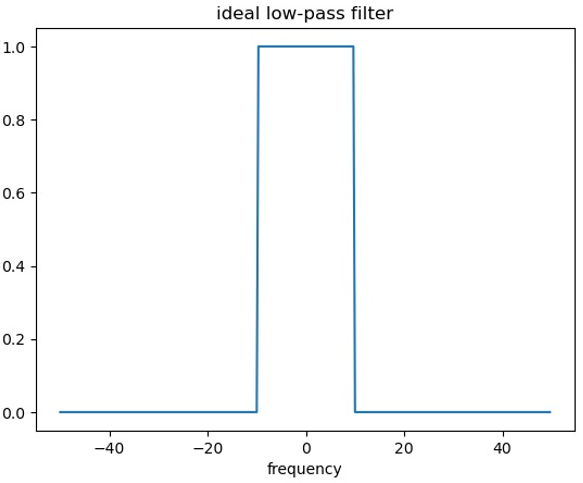
\includegraphics[width=0.28\textwidth]{Immagini/esfiltropassobasso1.png}
    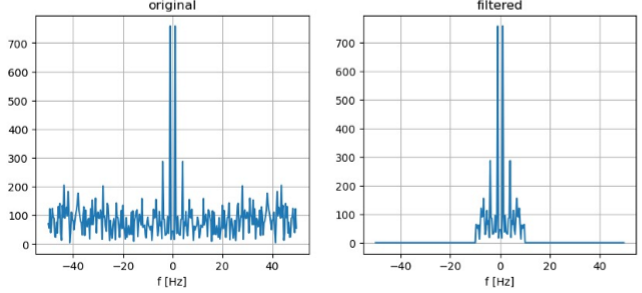
\includegraphics[width=0.5\textwidth]{Immagini/esfiltropassobasso2.png}
\end{center}
Il primo grafico è $H(\omega)$, il secondo è $F(\omega)$ e il terzo è $F_{\text{filt}}(\omega)$.
\subsection{Filtro Gaussiano}
Nel tempo:
\begin{equation*}
    g(t)=\frac{1}{\sqrt{2\pi}\sigma}e^{-\frac{t^{2}}{2\sigma^{2}}}
\end{equation*}
Nelle frequenze:
\begin{equation*}
    G(\omega)=e^{-\frac{\omega^{2}}{2\sigma^{2}_{f}}}
\end{equation*}
\begin{equation*}
    \sigma_{f}=\frac{1}{2\pi\sigma}
\end{equation*}
Non produce un taglio "netto" delle frequenze indesiderate, più $\sigma$ è grande più il taglia.\\
\textbf{Ricordo:} $\sum_{t}g(t)=1$
\begin{center}
    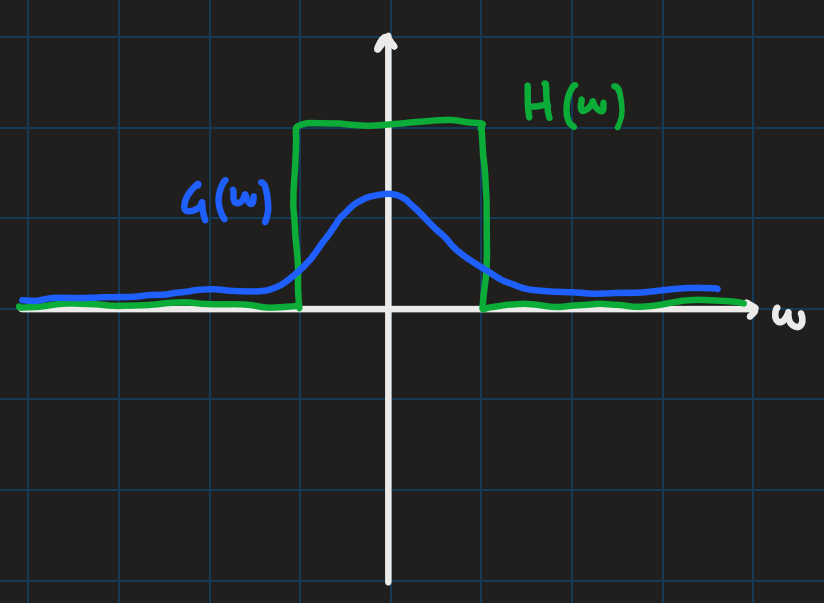
\includegraphics[width=0.7\textwidth]{Immagini/filtrogaussiano.png}
\end{center}
\subsection{Filtro Butterworth}
E' un filtro "liscio" ma con un cut-off più deciso
\begin{equation*}
    \lvert H(\omega) \rvert = \frac{1}{\lvert  B_{N}(i\frac{\omega}{\omega_{c}}) \rvert} = \frac{1}{\sqrt{1+\left(\frac{\omega}{\omega_{c}}\right)^{2N}}}
\end{equation*}
Più l'ordine $N$ è alto, più il cut-off $\left(\frac{\omega}{\omega_{c}}\right)$ è deciso.
\begin{center}
    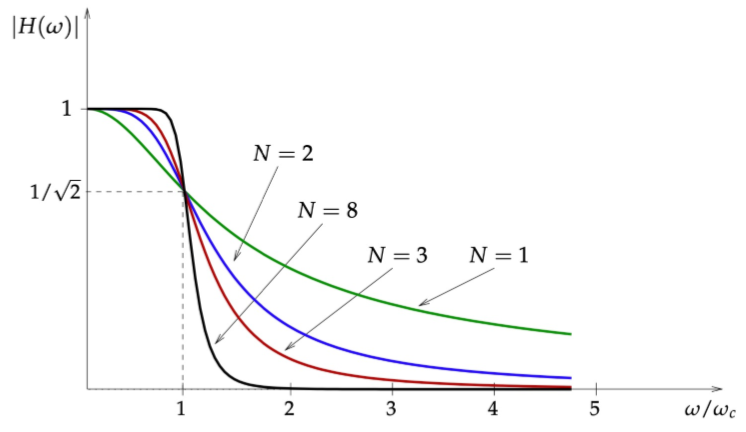
\includegraphics[width=0.7\textwidth]{Immagini/filtroButterworth.png}
\end{center}
\section{Rumore}
La riduzione del rumore avviene tramite filtraggio, di solito passa-alto.
\section{Filtraggio nel tempo}
\subsection{Convoluzione}
Consideriamo due funzioni continue $f(t)$ e $g(t)$, la loro convoluzione è definita come:
\begin{equation*}
    (f*g)(t) = \int_{-\infty}^{+\infty} f(\tau)g(t-\tau)d\tau
\end{equation*}
Dove la funzione $f$ è il filtro e $t$ è il tempo desiderato.\\
\underline{La convoluzione è commutativa: $f*g=g*f$}.
\subsection{Teorema di convoluzione}
\begin{equation*}
    f(t)*h(t) \iff F(\omega)H(\omega)
\end{equation*}
\begin{equation*}
    f(t)h(t) \iff F(\omega)*H(\omega)
\end{equation*}
In altre parole:
\begin{equation*}
    \tikzmark{ft}f(t)*\tikzmark{ht}h(t) = \tikzmark{ffilt}f_{\text{filt}}(t) \quad \tikzmark{Fo}F(\omega)\tikzmark{Ho}H(\omega) = \tikzmark{Ffilt}F_{\text{filt}}(t)
\end{equation*}
\begin{tikzpicture}[overlay, remember picture]
    \node (fte) [below of = ffilt, node distance = 4 em, anchor=west]{\footnotesize \textsf{FT}};
    \draw[-, in=180, out=-90] (ft.south)++(.25em,-.5ex) |- (fte.west);
    \draw[<-, in=180, out=-90] (Fo.south)++(.25em,-.5ex) |- (fte.east);
    \node (hte) [below of = ffilt, node distance = 3 em, anchor=west]{\footnotesize \textsf{FT}};
    \draw[-, in=180, out=-90] (ht.south)++(.25em,-.5ex) |- (hte.west);
    \draw[<-, in=180, out=-90] (Ho.south)++(.25em,-.5ex) |- (hte.east);
    \node (ffilte) [above right of = Fo, node distance = 2 em, anchor=west]{\footnotesize \textsf{IFT}};
    \draw[<-, in=180, out=-90] (ffilt.north)++(1em,2ex) |- (ffilte.west);
    \draw[-, in=180, out=-90] (Ffilt.north)++(1em,2ex) |- (ffilte.east);
\end{tikzpicture}
\subsection{Applicazioni tipiche}
\begin{itemize}
    \item \textbf{Ridurre il rumore} (filtri passa basso, nel tempo li chiamiamo filtri di smoothing)
    \item \textbf{Mettere in evidenza punti di cambiamento "rapido" del segnale} (filtri passa alto, nel tempo li chiamiamo filtri di enhancement)
\end{itemize}
\subsection{Convoluzione discreta}
Con $N$ punti nell'intervallo $[0,T]\rightarrow g[n]$, consideriamo un filtro $f[n]$
\begin{equation*}
    (f*g)[n] = \sum_{k=0}^{N-1} f[k]g[n-k] = \sum_{k=0}^{N-1} f[n-k]g[k]
\end{equation*}
Una pratica comune nel filtraggio digitale è quella di realizzare filtri di ampiezza finita $W$ (quello che ci interessa studiare) da utilizzare come maschere nell'operazione di filtraggio.
\subsection{Filtri di enhancement e differenze finite}
In matematica discreta le differenze finite sono definite come
\begin{equation*}
    f'(x) = \frac{f(x+h)-f(x)}{h}
\end{equation*}
Solitamente $h=1$.
\begin{center}
    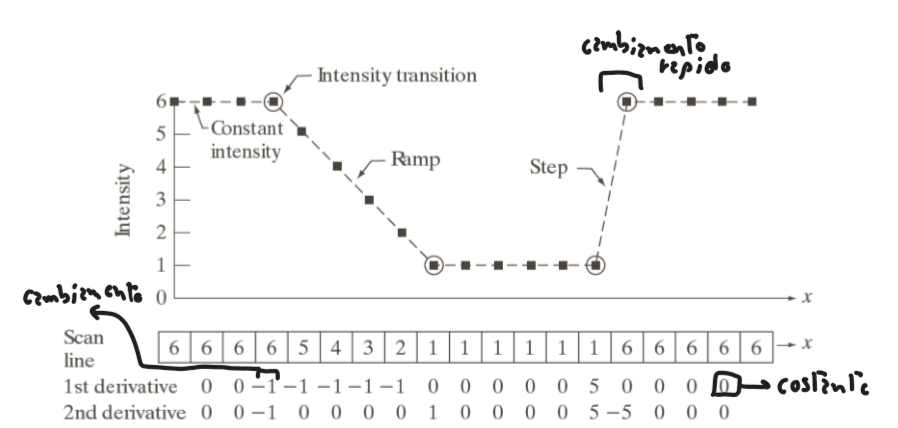
\includegraphics[width=0.8\textwidth]{Immagini/differenzefinite.png}
\end{center}
\subsection{Attenuazione del rumore}
Si può attenuare il rumore in un segnale usando un filtro passa basso e successivamente filtrare il segnale con un filtro passa alto per mettere in evidenza i punti di cambiamento. Esistono filtri che sono in grado di svolgere entrambi i compiti, per esempio la derivata della Gaussiana (che è una convoluzione tra Gaussiana e filtro passa alto). Il filtro mediano, in particolare, è utile a curare rumore impulsivo che si riscontra quando il segnale presenta valori errati e scorrelati dagli elementi vicini.
\chapter{Applicazione: Sound processing}
\section{Come nasce un segnale audio}
\begin{itemize}
    \item Il trasduttore elettroacustico (es. microfono) è in grado di tradurre le vibrazioni del suono in  un segnale elettrico
    \item Il convertitore Analogico-Digitale (ADC) lo trasforma in un segnale digitale applicando campionamento e quantizzazione
    \item Per l'ascolto è necessario seguire il procedimento opposto
    \item Alcuni segnali nascono direttamente da un dispositivo elettronico e quindi non necessitano il trasduttore iniziale
\end{itemize}
\section{Frequenza del suono}
L'unità di misura è l'Hertz (Hz) ed è il numero di vibrazioni al secondo.\\
L'altezza del suono dipende in gran parte dalle frequenze:
\begin{itemize}
    \item frequenze alte $\rightarrow$ suono acuto
    \item frequenze basse $\rightarrow$ suono grave
\end{itemize}
Per essere percepite come suono, le vibrazioni devono cadere all'interno di un intervallo compreso tra 20Hz e 20KHz, sopra i 20KHz sono ultrasuoni, sotto i 20Hz infrasuoni.\\
La gamma di suoni coperta dalla musica è molto più limitata (do grave 65 Hz, do acuto $\sim$8KHz)
\section{Campionamento}
\subsection{Teorema del campionamento}
Per ricostruire il segnale analogico occorre una frequenza di campionamento almeno doppia rispetto alla frequenza massima:
\begin{equation*}
    \frac{1}{\tau} > 2\omega_{\text{max}}
\end{equation*}
E per ottenere una ricostruzione "ragionevole" del segnale audio occorre una frequenza di campionamento almeno doppia rispetto alla frequenza massima udibile $\omega_{\text{max}}\geq 20\text{KHz}$
\section{Intensità del suono}
L'intensità del suono è legata all'ampiezza della vibrazione e si misura in decibel (DB), ha un range di "accettabilità" compreso tra:
\begin{itemize}
    \item Soglia di udibilità
    \item Soglia del dolore (130 DB)
\end{itemize}
\section{Short Time Fourier Transform (STFT)}
Un limite della trasformata di Fourier è che descrive il contenuto "globale" del segnale in termini di frequenza, ma non ci permette di localizzare un fenomento all'interno del segnale (in altre parole: perdo l'ordine nel tempo in cui vengono eseguite le cose).
\begin{itemize}
    \item Invece di considerare l'intero segnale, consideriamo porzioni del segnale
    \item I risultati ottenuti dipendono dalla dimensione dellaa finestra
    \item Dipendono anche dalla forma (tagli bruschi introducono artefatti)
    \item La STFT può essere invertita
\end{itemize}
\section{Spettrogrammaa}
E' una rappresentazione bidimensionale del modulo della STFT
\begin{center}
    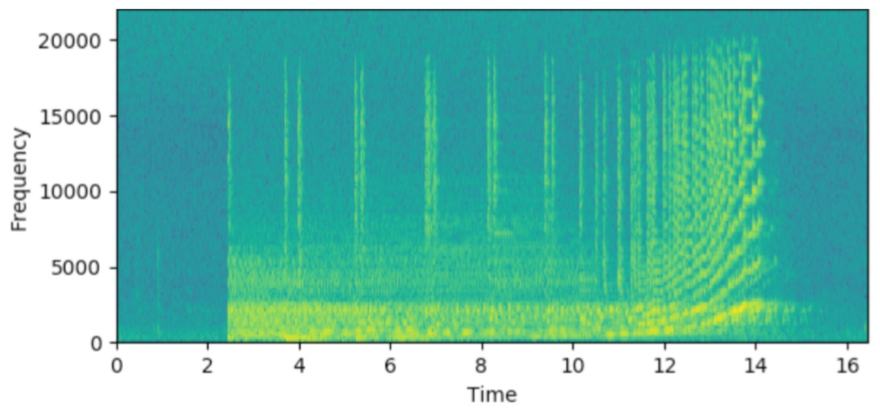
\includegraphics[width=.8\textwidth]{Immagini/spettrogramma.png}
\end{center}
\chapter{Immagini digitali}
\end{document}